\begin{figure}[htbp]
    \centering
    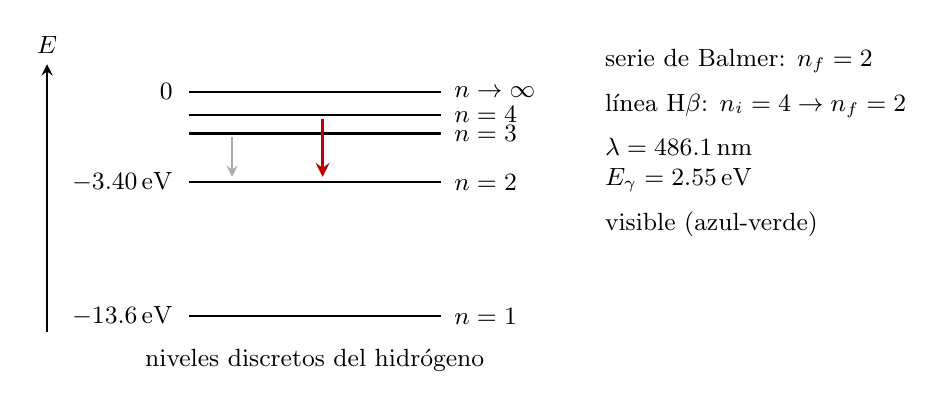
\begin{tikzpicture}[>=stealth, every node/.style={font=\small}]
        \draw[->,thick] (0,0.15) -- (0,3.55) node[above] {$E$};
        \draw[thick] (1.8,0.35) -- (5.0,0.35);
        \draw[thick] (1.8,2.05) -- (5.0,2.05);
        \draw[thick] (1.8,2.67) -- (5.0,2.67);
        \draw[thick] (1.8,2.91) -- (5.0,2.91);
        \draw[thick] (1.8,3.2) -- (5.0,3.2);
        \node[left,align=right] at (1.72,0.35) {$-13.6\,\mathrm{eV}$};
        \node[left,align=right] at (1.72,2.05) {$-3.40\,\mathrm{eV}$};
        \node[left,align=right] at (1.72,3.2) {$0$};
        \node[right] at (5.05,0.35) {$n=1$};
        \node[right] at (5.05,2.05) {$n=2$};
        \node[right] at (5.05,2.67) {$n=3$};
        \node[right] at (5.05,2.91) {$n=4$};
        \node[right] at (5.05,3.2) {$n\to\infty$};

        \draw[->,very thick,red!75!black] (3.5,2.86) -- (3.5,2.12);
        \draw[->,thick,gray!65] (2.35,2.63) -- (2.35,2.12);
        \node[align=left] at (9.0,2.55)
            {serie de Balmer: $n_f=2$\\[5pt]
             línea H$\beta$: $n_i=4\to n_f=2$\\[5pt]
             $\lambda=486.1\,\mathrm{nm}$\\
             $E_\gamma=2.55\,\mathrm{eV}$\\[5pt]
             visible (azul-verde)};
        \node[below] at (3.4,0.05) {niveles discretos del hidrógeno};
    \end{tikzpicture}
    \caption{Niveles de energía del hidrógeno y transiciones hacia $n_f=2$. La flecha roja indica la línea H$\beta$ observada en la nebulosa.}
    \label{fig:serie-balmer}
\end{figure}